\section{Auswertung}

Die Formel für den Mittelwert lautet
 \begin{equation}
    \bar{x}=\frac{1}{n}\sum_{i=1}^n x_i.\\
\end{equation}
Die Standardabweichung wird mit folgender Formel
\begin{equation}
    s_x=\sqrt{\frac{1}{n-1}\sum_{i=1}^n {(x_i-\bar{x})^2 }}\\
\end{equation}
berechnet.
Die Formel für den Fehler des Mittelwertes lautet
\begin{equation}
    \Delta \bar{x} = s_{\bar{x}}=\frac{s_x}{\sqrt{n}}= \sqrt{\frac{1}{n(n-1)}\sum_{i=1}^n {(x_i-\bar{x})^2 }}.\\
\end{equation}
Diese werden im Folgenden verwendet.

\subsection{Bestimmung der Untergrundrate}
Die Untergrundrate $N_U$ wird mehrfach gemessen mit dem Messintervall $ \Delta t=300 \text{s}$.\\
Die Messwerte von $N_U$ betragen =$\{129, 143, 144, 136, 139, 126, 158\}$ Imp.\\
Der Untergrund $N_U$ wird mit der Formel
\begin{equation}
  N_U = \frac{\bar{{N_U}}}{\Delta t} \\
 \end{equation}
 bestimmt.
Der Untergrund ergibt 
\begin{align*}
  N_U= ( 0,464 \pm 0,033) \, \mathrm{Imp}.\\
\end{align*}
\noindent
Der Untergrund (Anzahl der Impulsen bei der ohne Probe erhältlichen Zählrohr) werden bei der folgenden Teilen des Versuches von den Zählraten abgezogen.
\newpage
\subsection{Bestimmung der Halbwertszeit von Vanadium}

Die aktivierte Vanadiumprobe wird direkt nach dem Entnehmen aus der Neutronenquelle auf das Geiger-Muller-Zahlrohr gesteckt,
 dann wird die Messung gestartet. Als Messintervall wird $\Delta t =30 \text{s}$ gewählt.
Die Nullräten werden aus den gemessen Zählraten mit  Formel
\begin{equation}
  N = N_\text{mess}-N_U \cdot \Delta t \\
 \end{equation}
 abgezogen und die Fehler der Zählraten werden mit Formel
 \begin{equation}
  \Delta N = \sqrt{N}\\
 \end{equation}
 berechnet.\\
 Diese Messwerte und berechneten Werte sind in Tabelle \ref{tab:Vanadium} (siehe \ref{sec:Anhang}) aufgelistet. \\
Die Zerfallskurve der Vanadiumprobe wird in Grafik \ref{fig:Vanadium} veranschaulicht.
\begin{figure}[H]
  \centering
  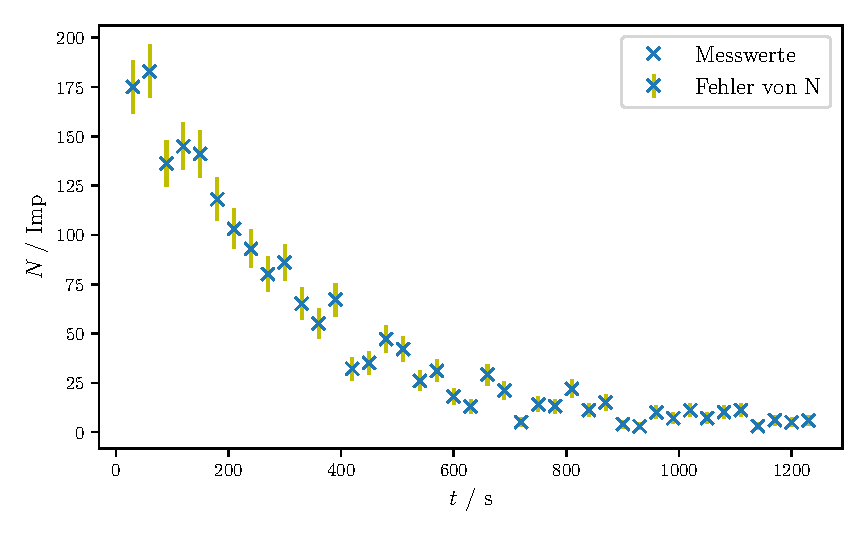
\includegraphics{Vanadium.pdf}
  \caption{Die Zerfallskurve der Vanadiumprobe.}
  \label{fig:Vanadium}
\end{figure}
\noindent
Da die letzten Zahlintervalle sehr geringe Zahlraten haben, wird die Bestimmung der Zerfallszeit  dadurch sehr ungenau.
Deswegen werden nur die Messwerte verwendet, die im Zeitintervall von 0 bis 540 s gemessen werden.
In diesem Zeitintervall wird eine lineare Regression hinzugeführt.
Die Ausgleichsgerade besitz die Form:
\begin{equation}
 \text{ln}(N)=-a\cdot t+b \\
\end{equation}
mit \(a= \lambda\), \(b=\text{ln}(N_{t=0})(1-e^{\lambda \Delta t})\).\\
Die Parameter ergeben 
\begin{align*}
  a &=(3,724 \pm0,246 ) \cdot 10^{-3}\,\mathrm{\frac{1}{s}} \\
  b &=(5,400 \pm0,097 ) .\\
 \end{align*}
\noindent Daraus ergibt sich die Halbwertszeit von Vanadidum 
 \begin{equation}
 T= \frac{\text{ln}2}{\lambda}= (186,130 \pm 12,295)\,\mathrm{s}.\\
 \end{equation}
 \noindent Zur Bestimmung der Zerfallskonstante $\lambda$ und Halbwertszeit $T$ der Vanadiumprobe wird eine Die Ausgleichungsgerade hinzugeführt.
  Diese wird in Abbildung \ref{fig:Vanadiumausgleichung} dargestellt. 
\begin{figure}[H]
  \centering
  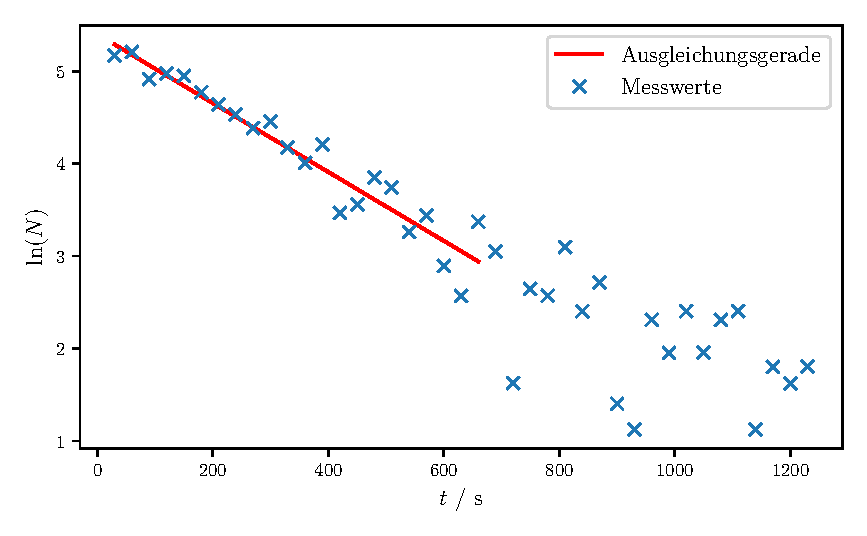
\includegraphics{Vanadiumausgleichung.pdf}
  \caption{Die Ausgleichungskurve zur Bestimmung der Zerfallskonstante und Halbwertszeit der Vanadiumprobe.}
  \label{fig:Vanadiumausgleichung}
\end{figure}


\subsection{Bestimmung der Halbwertszeit von Rhodium}
Die Messung wird analog zu der Messung mit Vanadium durchgefuhrt. Der Messintervall beträgt bei Rhodium $\Delta t= 15\,s$.
Diese Messwerte und berechneten Werte sind in Tabelle \ref{tab:Rhodium} (siehe \ref{sec:Anhang}) aufgelistet. \\
Die Zerfallskurve der Rhodiumprobe wird in Grafik \ref{fig:Rhodium} veranschaulicht.
\begin{figure}[H]
  \centering
  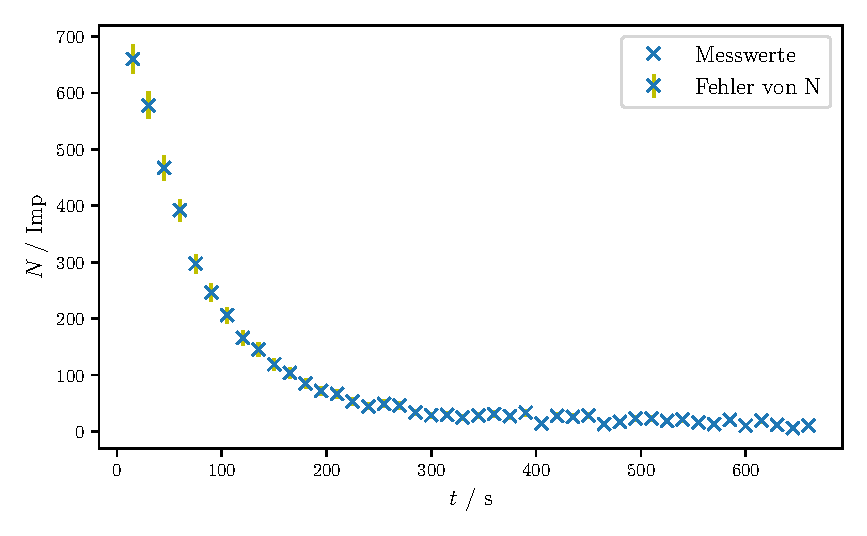
\includegraphics{Rhodium.pdf}
  \caption{Die Zerfallskurve der Rhodiumprobe.}
  \label{fig:Rhodium}
\end{figure}
\noindent Die Ausgleichungskurven zur Bestimmung der Zerfallskonstante $\lambda$ und Halbwertszeit $T$ der Rhodiumprobe werden in Grafik \ref{fig:Rhodiumausgleichung} veranschaulicht.
\begin{figure}[H]
  \centering
  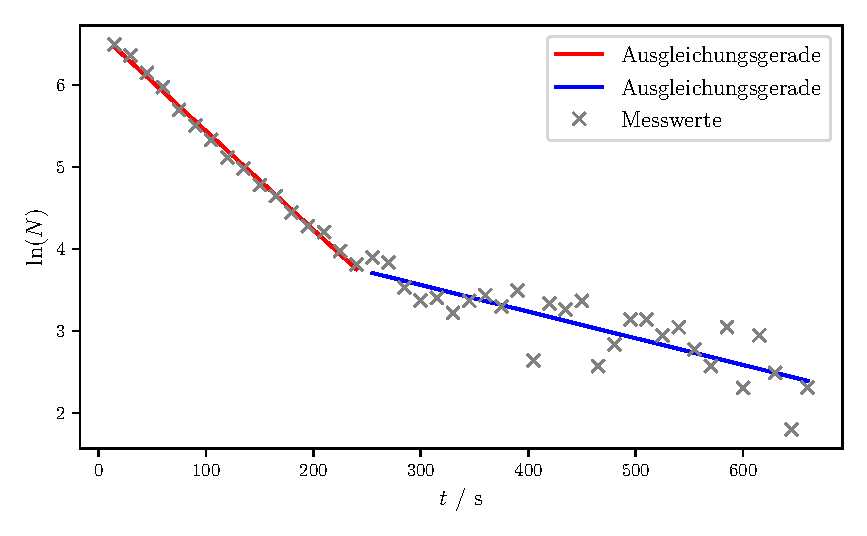
\includegraphics{Rhodiumausgleichung.pdf}
  \caption{Die Ausgleichungskurven zur Bestimmung der Zerfallskonstante und Halbwertszeit der Rhodiumprobe.}
  \label{fig:Rhodiumausgleichung}
\end{figure}
\noindent Wie aus der Abbildung \ref{fig:Rhodium} hervorgeht, besteht die Probe nicht aus einem einzelnen radioaktiven Nuklid, sondern
aus zwei unabhängig zerfallenden Nukliden.
In diesem Zeitintervall werden die lineare Regressionen hinzugeführt.\\
Die Ausgleichsgerade besitz die Form:
\begin{equation}
 \text{ln}(N)=-a_{1,2}\cdot t+b_{1,2}\\ 
\end{equation}
mit \(a_{1,2}= \lambda_{1,2}\), \(b_{1,2}=\text{ln}(N_{t=0})(1-e^{\lambda_{1,2} \Delta t})\).\\
Die Parameter ergeben 
\begin{align*}
  a_1 &=(12,035 \pm0,207) \cdot 10^{-3}\,\mathrm{\frac{1}{s}} \\
  b_1 &=(6,641\pm0,030 ) .\\
  a_2 &=(3,249 \pm0,430) \cdot 10^{-3}\,\mathrm{\frac{1}{s}} \\
  b_2 &=(4,535\pm0,204 ) .\\
 \end{align*}
\noindent 
\newpage
\noindent Aus den Steigungen $a_1$ und $a_2$ der beiden eingezeichneten Geraden lassen sich näherungsweise die Halbwertszeiten $T_{1,2}$ (entspricht dem kurzlebigen und langlebigen  Zerfall)
\begin{align*}
 T_1 &= (57,594 \pm 0,991)\,\mathrm{s} \\
 T_2 &= (213,341 \pm 28,235)\,\mathrm{s}\\
\end{align*}
bestimmen.

\label{sec:Auswertung}
